\subsection{Allgemeines}
\label{subsec:pofallgemeines}

Optische Wellenleiter, auch Lichtwellenleiter genannt, verwenden Licht zur
Übertragung von Informationen. Dies ermöglicht eine schnellere Datenübertragung
als mit Kupferkabeln. Glasfaserkabel werden mittlerweile für die Verbindung von
Städten und Kontinenten, aufgrund ihrer hohen Reichweite von mehreren Kilometern
und der hohen Übertragungsleistung von bis zu 32 Gigabit/s pro Kabel,
eingesetzt. Die Anbindung von Gebäuden und Wohnungen an das Glasfaserkabelnetz
ist mittlerweile ein erklärtes Ziel der Telekommunikationsunternehmen. Durch
Projekte wie \shorthandoff{"}"Fiber to the Home"\shorthandon{"} oder
\shorthandoff{"}"Fiber to the Building"\shorthandon{"} sollen Privatpersonen und
Unternehmen von den hohe Übertragungsgeschwindigkeiten profitieren. Jedoch sind
Glasfaserkabel für die Verlegung in Gebäuden ungeeignet, da diese nur durch
Fachpersonal mit Spezialwerkzeug vorgenommen werden kann und relativ teuer ist
\cite{poflan}. Polymer optische Fasern (POF) bieten sich hier als kostengünstige
Alternative an. Sie lassen sich einfach und platzsparend verlegen (der
Durchmesser beträgt ca. 1 mm) und auf kurzen Distanzen (< 100 m) können
Datenraten von bis zu 40 Gigabit/s \cite{pofacgif} erreicht werden (bei
zunehmender Entfernung nimmt die Datenkapazität ab) \cite{pofacprofile}.
POF-Kabel werden nicht nur für den Anschluss an das Internet eingesetzt, sondern
auch in Flugzeugen, Zügen, Automobilen und Industrieanlagen.
\autoref{fig:pofgrund} zeigt die Gründe für die Verwendung in dem jeweiligen
Bereich.

\begin{figure}[h]
    \begin{center}
        \begin{minipage}[t]{\textwidth}
            \begin{center}
                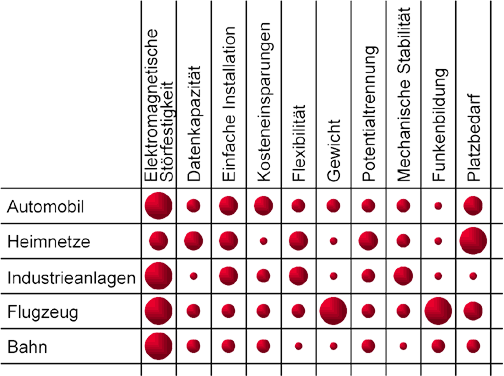
\includegraphics[height=0.2\textheight]{Bilder/Optische_Wellenleiter_Die_Polymer_Optische_Faser/Allgemeines/pofgrund.png}
                \caption[Gründe für die Verwendung von POF-Kabel \newline \url{http://www.pofac.fh-nuernberg.de/pofac/de/was_sind_pof/images/warum_pof.png} (zuletzt aufgerufen am 19.09.2015)]{Gründe für die Verwendung von POF-Kabel}
                \label{fig:pofgrund}
            \end{center}
        \end{minipage}
    \end{center}
\end{figure}

Die Größe des Kreisradius in der jeweiligen Zelle zeigt die Relevanz des
Kriteriums an.

Elektromagnetische Strahlung, elektrische Felder und Magnetfelder,
beeinträchtigen den Fluss von Elektronen in Kupferkabeln, jedoch nicht den von
Lichtstrahlen in einem Lichtwellenleiter. Daher kommen polymer optische Fasern
für die Verbindung der Sensorik zum Einsatz, da eine Störung der
Datenübertragung fatale Folgen haben könnte. Bei Flugzeugen spielen das Gewicht
und die Funkenbildung ebenfalls eine große Rolle. Durch das geringe Gewicht von
POF-Kabel reduziert sich der Treibstoffverbrauch und damit die Betriebskosten.
Polymer optische Fasern übertragen im Gegensatz zu einem Kupferkabel keine
Elektronen sondern Licht und können somit keine Funken bilden - eine mögliche
Gefahrenquelle eliminiert. Weitere Einsatzmöglichkeiten findet man in
Krankenhäusern, da POFs keine elektromagnetische Strahlung emittieren, werden
empfindliche Messgeräte nicht gestört.
